\subsection{Sensitivity and the device specification sheet}\label{sec:spec}
\paragraph{Design.} Around a protonic-like base device we move one parameter at a time while keeping the others at the base:
\begin{itemize}
\item the base: 1000 levels, asymmetry 0.05, saturation 0.2, write noise 0.3, no drift, reference error 0.02;
\item the parameters moved: levels, asymmetry, nonlinearity (saturation $\gamma$), write noise, retention and reference error;
\item the algorithm: the pre-registered TTv2, our best validation choice, at the FP learning rate;
\item the sizes: three CIFAR and three LM sizes, with SGD at the base sizes.
\end{itemize}
Fig.~\ref{fig:oat} shows the curves.

\paragraph{The pre-registered sheet degenerates.} The rule asks for the weakest value that keeps the gap under the line. On
CIFAR, the base device's own TTv2 gap at the FP rate is already near or above the line:
\RSpecrelTtvTwoCifarWOneSixBasegap, \RSpecrelTtvTwoCifarWThreeTwoBasegap{} and \RSpecrelTtvTwoCifarWSixFourBasegap\,pp at
$c=16$, 32 and 64. Most CIFAR entries therefore read ``not reachable'' (Table~\ref{tab:spec}). Two things cause this: the CIFAR
baseline's seed noise (Section~\ref{sec:main}) and TTv2's need for its own learning rate at larger widths
(Section~\ref{sec:scale}). On the LM at $d=64$ and 128 the base passes and the sheet is well defined.

\paragraph{Degradation thresholds.} We therefore add a descriptive reading, labelled as added after the data were seen
(\texttt{DEVIATIONS-PAPER.md} D1): how far each parameter may move before the gap rises by more than the line over the base
device's own gap (Table~\ref{tab:specrel}). Its main features are consistent across sizes and tasks:

\begin{description}
\item[Reference error is the binding specification.] With the symmetry-point reference exact ($\sigma_r=0$) the TTv2 gap
      vanishes: \ROatTtvTwoCifarWThreeTwoReferrzero\,pp on CIFAR and \ROatTtvTwoLmWOneTwoEightReferrzero\% on the LM at the base
      sizes. Already at $\sigma_r=0.05$ it reaches \ROatTtvTwoCifarWThreeTwoReferrfive\,pp and
      \ROatTtvTwoLmWOneTwoEightReferrfive\%. At every size the grid threshold is $\sigma_r$ \RSpecrelTtvTwoCifarWThreeTwoRefErr{} of the half-range;
      the interpolated crossings lie just above it (Table~\ref{tab:specrel}).
      This is the offset sensitivity that c-TTv2 and AGAD were designed to remove~\cite{rasch2024}. Their better main-table
      results (Section~\ref{sec:main}) and our validation (Section~\ref{sec:validation}) say that a specification sheet for
      them would relax this line.
\item[The device must saturate.] A constant-step device ($\gamma=0$) fails badly under TTv2
      (\ROatTtvTwoCifarWThreeTwoGammazero\,pp; \ROatTtvTwoLmWOneTwoEightGammazero\%), as~\cite{rasch2024} predicts for algorithms
      that rely on the device's own decay toward its symmetry point. Up to $\gamma\approx0.5$ is tolerated.
\item[Asymmetry up to about 0.2] is tolerated. At 0.4 training collapses (\ROatTtvTwoCifarWThreeTwoAsymfour\,pp).
\item[Levels matter less than expected.] TTv2 tolerates a few hundred levels: the threshold is \RSpecrelTtvTwoCifarWThreeTwoNStates{}
      on CIFAR at $c=32$ and \RSpecrelTtvTwoLmWOneTwoEightNStates{} on the LM at $d=128$. With 100 levels the gap is
      \ROatTtvTwoCifarWThreeTwoLevelshundred\,pp and \ROatTtvTwoLmWOneTwoEightLevelshundred\%. This is far below the thousand
      levels plain SGD needs~\cite{gokmen2016}.
\item[Write noise] up to one to two steps per pulse is tolerated. Four steps hurts (\ROatTtvTwoCifarWThreeTwoCtwocfour\,pp;
      \ROatTtvTwoLmWOneTwoEightCtwocfour\%).
\item[Retention.] The drift time constant must be \RSpecrelTtvTwoLmWOneTwoEightTauSteps{} training steps on the LM ($d=128$)
      and \RSpecrelTtvTwoCifarWThreeTwoTauSteps{} on CIFAR ($c=32$). That is
      several to tens of times the length of our training runs, which are 2340 and 3000 steps. At $10^3$ steps training fails
      (\ROatTtvTwoCifarWThreeTwoTauthree\,pp; \ROatTtvTwoLmWOneTwoEightTauthree\%). For a real array the required time is this
      number of steps times the update time per step.
\item[Plain SGD] stays far above the line at every point of the grid on both tasks. No single parameter, moved alone from a
      protonic-like device, makes plain SGD work.
\end{description}

\paragraph{Pairs and the joint specification.} \RPairSentence{} On both tasks the six largest interactions all pair the shortest
retention ($\tau=10^3$ steps) with a second imperfection. A drifting device compounds every other error, so retention must be
specified jointly with the rest. Away from fast drift, the pairwise effects are close to additive. The joint specification, with every parameter at its threshold
at once (Table~\ref{tab:spec}, last column), \RJointSentence

% generated by analyze.py (do not edit)
\begin{table*}[t]\centering\footnotesize\caption{Device specification sheet (E5) for TTv2: the weakest grid value of each parameter that keeps the gap under the line (2 pp CIFAR; 5\% LM) with every other parameter at the protonic base (levels 1000, $a$ 0.05, $\gamma$ 0.2, $c_{2c}$ 0.3, no drift, $\sigma_r$ 0.02); in parentheses the interpolated crossing. $^\dagger$: the base itself fails and the value shown is the improvement needed; $^*$: passes over the whole grid; n/r: not reachable on the grid. Last column: the joint specification (every axis at its threshold at once), mean gap over 3 seeds, round 1 or the tightened round 2.}\label{tab:spec}
\fitbox{\begin{tabular}{lccccccc}\toprule Size & Levels & Asym.\ $a$ & Nonlin.\ $\gamma$ & Noise $c_{2c}$ & Retention $\tau$ & Ref.\ err.\ $\sigma_r$ & Joint spec\\\midrule
CIFAR 16 & n/r & n/r & n/r & n/r & n/r & $\le$ 0 (0.0104)$^\dagger$ & --\\
CIFAR 32 & $\ge$ 2000 (1488)$^\dagger$ & n/r & n/r & $\le$ 0 (0.17)$^\dagger$ & n/r & $\le$ 0 (0.0179)$^\dagger$ & --\\
CIFAR 64 & n/r & n/r & n/r & n/r & n/r & n/r & --\\
LM 64 & $\ge$ 500 (292) & $\le$ 0.2 (0.231) & $\le$ 0.2 (0.379) & $\le$ 1 (1.12) & $\ge$ 1e4 (7e3) & $\le$ 0.02 (0.0239) & r1: 4.74 pass\\
LM 128 & $\ge$ 1000 (612) & $\le$ 0.2 (0.21) & $\le$ 0.2 (0.281) & $\le$ 0.3 (0.727) & $\ge$ 1e4 (8e3) & $\le$ 0.02 (0.021) & r1: 2.45 pass\\
LM 256 & n/r & n/r & n/r & n/r & n/r & n/r & --\\
\bottomrule\end{tabular}}\end{table*}

% generated by analyze.py (do not edit)
\begin{table*}[t]\centering\footnotesize\caption{Degradation thresholds (descriptive, added after the one-at-a-time data were seen; DEVIATIONS-PAPER.md D1): the weakest grid value of each parameter whose gap stays within the line (2 pp CIFAR; 5\% LM) of the protonic base device's own gap (column 3), all other parameters at the base; interpolated crossing in parentheses; $^*$ the whole grid stays within; n/r the nearest grid step already leaves the band.}\label{tab:specrel}
\fitbox{\begin{tabular}{llrcccccc}\toprule Alg. & Size & Base gap & Levels & Asym.\ $a$ & Nonlin.\ $\gamma$ & Noise $c_{2c}$ & Retention $\tau$ & Ref.\ err.\ $\sigma_r$\\\midrule
SGD & CIFAR 32 & 19.80 & $\ge$ 1000 (520) & $\le$ 0.05 (0.0813) & $\le$ 0.2 (0.266) & $\le$ 1 (1.3) & $\ge$ 1e4 (7e3) & $\le$ 0.1 (0.15)\\
SGD & LM 128 & 39.85 & $\ge$ 200 (143) & $\le$ 0.4$^*$ & $\le$ 0.2 (0.423) & $\le$ 4$^*$ & $\ge$ 1e4 (3e3) & $\le$ 0.5$^*$\\
TTv2 & CIFAR 16 & 4.03 & $\ge$ 100$^*$ & $\le$ 0.2 (0.204) & $\le$ 0.5 (0.606) & $\le$ 0.3 (0.789) & $\ge$ 1e5 (7e4) & $\le$ 0.02 (0.0228)\\
TTv2 & CIFAR 32 & 2.39 & $\ge$ 500 (265) & $\le$ 0.2 (0.209) & $\le$ 0.5 (0.578) & $\le$ 2 (2.31) & $\ge$ 1e5 (2e4) & $\le$ 0.02 (0.0241)\\
TTv2 & CIFAR 64 & 7.32 & $\ge$ 100$^*$ & $\le$ 0.2 (0.203) & $\le$ 2$^*$ & $\le$ 2 (2.62) & $\ge$ 1e5 (4e4) & $\le$ 0.02 (0.0244)\\
TTv2 & LM 64 & 3.18 & $\ge$ 200 (130) & $\le$ 0.2 (0.284) & $\le$ 0.5 (0.717) & $\le$ 2 (2.03) & $\ge$ 1e4 (5e3) & $\le$ 0.02 (0.0326)\\
TTv2 & LM 128 & 4.25 & $\ge$ 200 (167) & $\le$ 0.2 (0.276) & $\le$ 0.5 (0.705) & $\le$ 1 (1.67) & $\ge$ 1e4 (6e3) & $\le$ 0.02 (0.028)\\
TTv2 & LM 256 & 16.29 & $\ge$ 100$^*$ & $\le$ 0.4$^*$ & $\le$ 2$^*$ & $\le$ 2 (2.64) & $\ge$ 1e4 (4e3) & $\le$ 0.02 (0.0351)\\
\bottomrule\end{tabular}}\end{table*}

% generated by analyze.py (do not edit)
\begin{table}[t]\centering\footnotesize\caption{Pairwise sensitivity (E5): the three largest interactions per task, interaction = gap(a,b) $-$ [gap(a) + gap(b) $-$ gap(base)].}\label{tab:pairs}
\fitbox{\begin{tabular}{llccc}\toprule Task & Pair & Gap(a,b) & Singles & Interaction\\\midrule
CIFAR & asym=0.1, tau\_steps=1e3 & 46.64 & 1.82 + 33.96 & 13.25\\
CIFAR & asym=0.2, tau\_steps=1e3 & 40.24 & 1.92 + 33.96 & 6.75\\
CIFAR & gamma=0.5, tau\_steps=1e3 & 41.17 & 3.55 + 33.96 & 6.05\\
LM & c2c=1, tau\_steps=1e3 & 76.94 & 5.27 + 33.74 & 42.18\\
LM & gamma=0.5, tau\_steps=1e3 & 76.63 & 6.28 + 33.74 & 40.85\\
LM & asym=0.1, tau\_steps=1e3 & 73.70 & 4.09 + 33.74 & 40.11\\
\bottomrule\end{tabular}}\end{table}

\begin{figure}[t]\centering
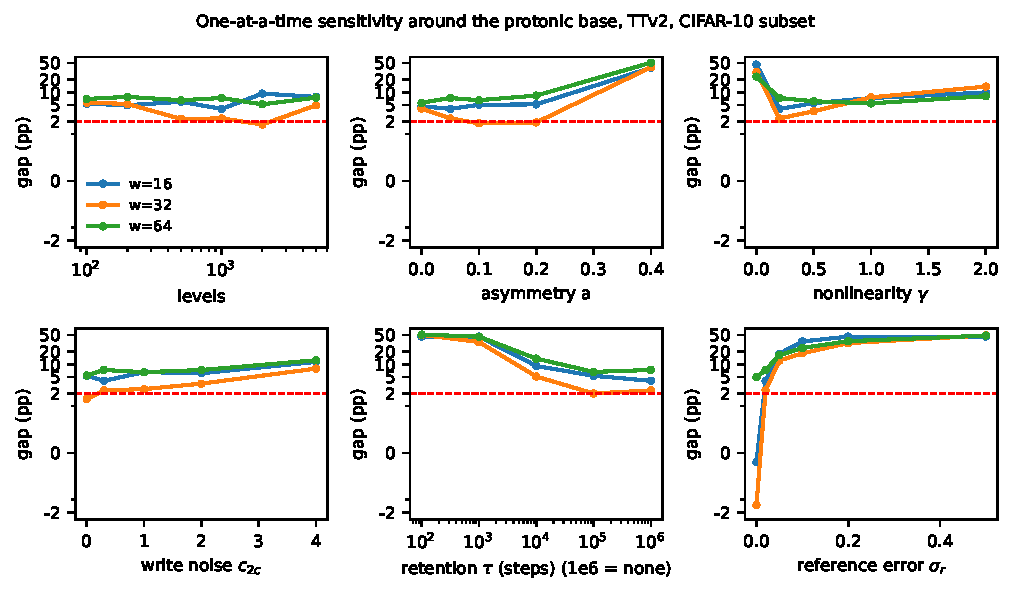
\includegraphics[width=\linewidth]{figs/fig_oat_cifar}
\caption{One-at-a-time sensitivity around the protonic base device on the CIFAR-10 subset (TTv2 at the FP learning rate;
seed 0, plus seed 1 near the line): gap against each parameter at three widths; dashed: the gap line.}\label{fig:oat}
\end{figure}
\begin{figure}[t]\centering
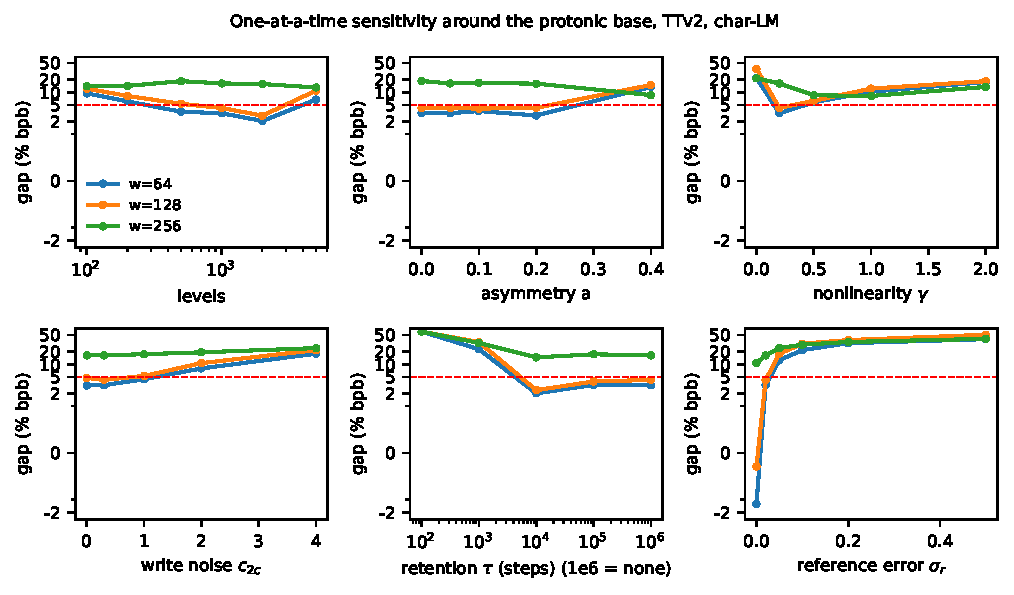
\includegraphics[width=\linewidth]{figs/fig_oat_lm}
\caption{As Fig.~\ref{fig:oat}, for the character LM.}\label{fig:oatlm}
\end{figure}
